\section{Data Description and Visualisation}

The dataset used in this assignment consists of meteorite compositional data. Specifically, it contains 12 samples collected from different geographical locations (see Fig.~\ref{fig:locations_som_convexhull}). Each sample records the composition across nine parts: the metal oxides \{FeO, Al$_2$O$_3$, MgO, SiO$_2$, MnO\}, the metals \{Fe, Ni, Co\}, and carbon (C). In addition to the compositional data, each sample is associated with a chondrite type, summarized in Table~\ref{tab:chondrite-types}.

\begin{table}[H]
\centering
\begin{tabular}{@{}ll@{}}
\toprule
\textbf{Code} & \textbf{Meaning} \\ \midrule
cc & \textbf{Carbonaceous chondrite}: rich in carbon, hydrated minerals, primitive, volatile-rich. \\
hc & \textbf{High-iron chondrite} (H chondrite): ordinary chondrite with high metal content. \\
lc & \textbf{Low-iron chondrite} (L chondrite): ordinary chondrite with lower metal content. \\ \bottomrule
\end{tabular}
\caption{Summary of meteorite chondrite types and their meanings.}
\label{tab:chondrite-types}
\end{table}

It is important to note that the raw compositional data are not closed (i.e., they do not sum to a constant value such as 100). For the purposes of this analysis, all compositions were closed to a total sum of 100, a standard preprocessing step for compositional data. This transformation ensures that the data adhere to the properties of compositional space, where only the relative proportions between components carry meaningful information.

Additionally, the data exhibit key features typical of compositional datasets: the dominance of certain components (e.g., SiO$_2$, FeO, and MgO) and the inherently relative nature of the measurements, where increases in one part necessarily imply decreases in others due to the constant sum constraint.

To provide an overview of the data, a stacked bar plot was created for each sample, shown in Fig.~\ref{fig:stacked}, after applying closure to 100. Visual inspection of this plot reveals substantial variation in the abundance of certain parts across samples, while components like SiO$_2$, FeO, and MgO consistently make up the majority of the overall composition regardless of sample.

To further explore compositional similarities between samples, a clustermap was generated (Fig.~\ref{fig:clustermap}). This visualisation highlights patterns such as the clustering of samples Bali and Allende, which stand out due to their high metal content, and the distinct position of Kabo, characterized by a notably high carbon content.


\begin{figure}[htbp]
    \centering
    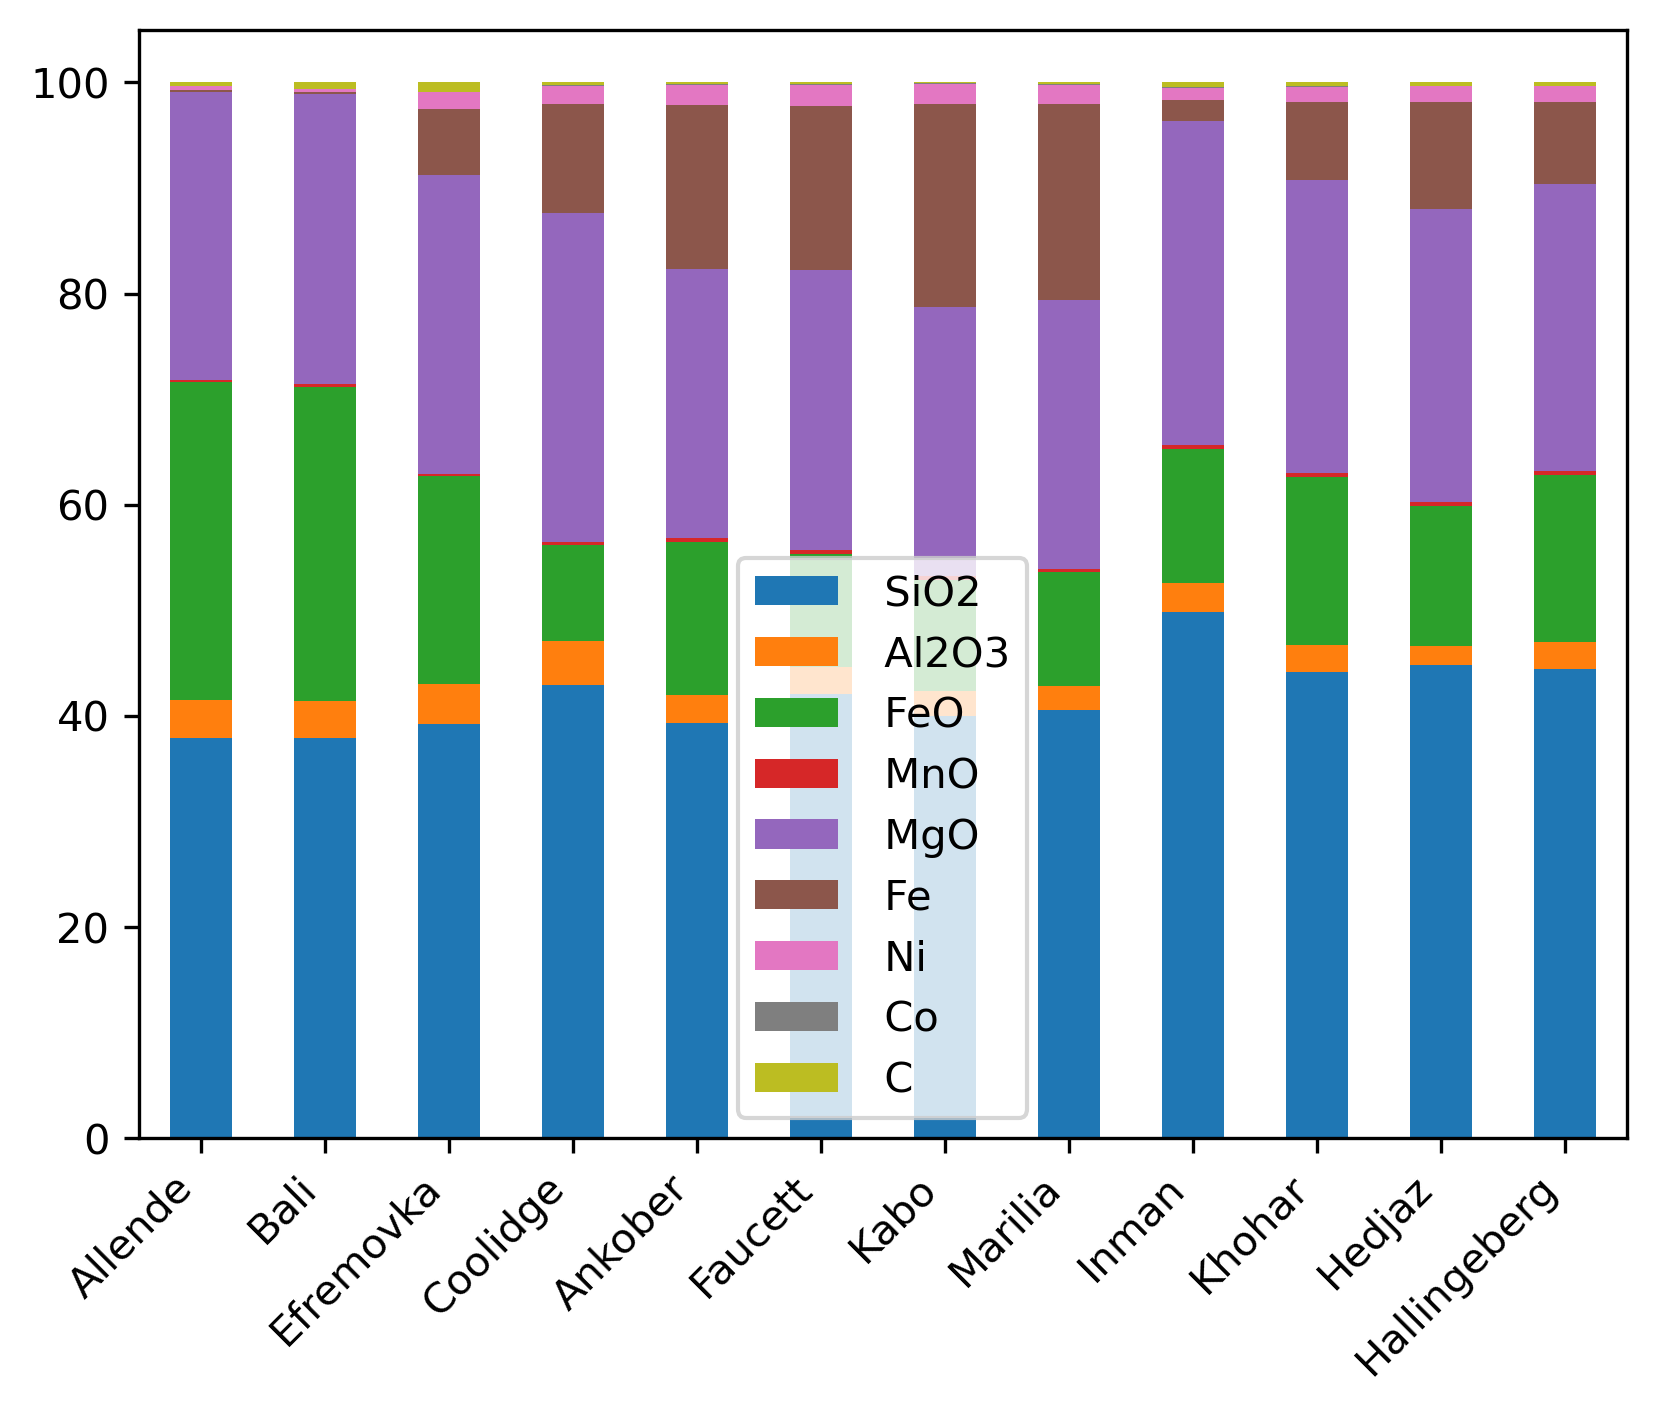
\includegraphics[width=0.8\textwidth]{figures/stacked_bar.png}
    \caption{Example plot showing the chemical composition of meteorites.}
    \label{fig:stacked}
\end{figure}



\begin{figure}[H]
    \centering
    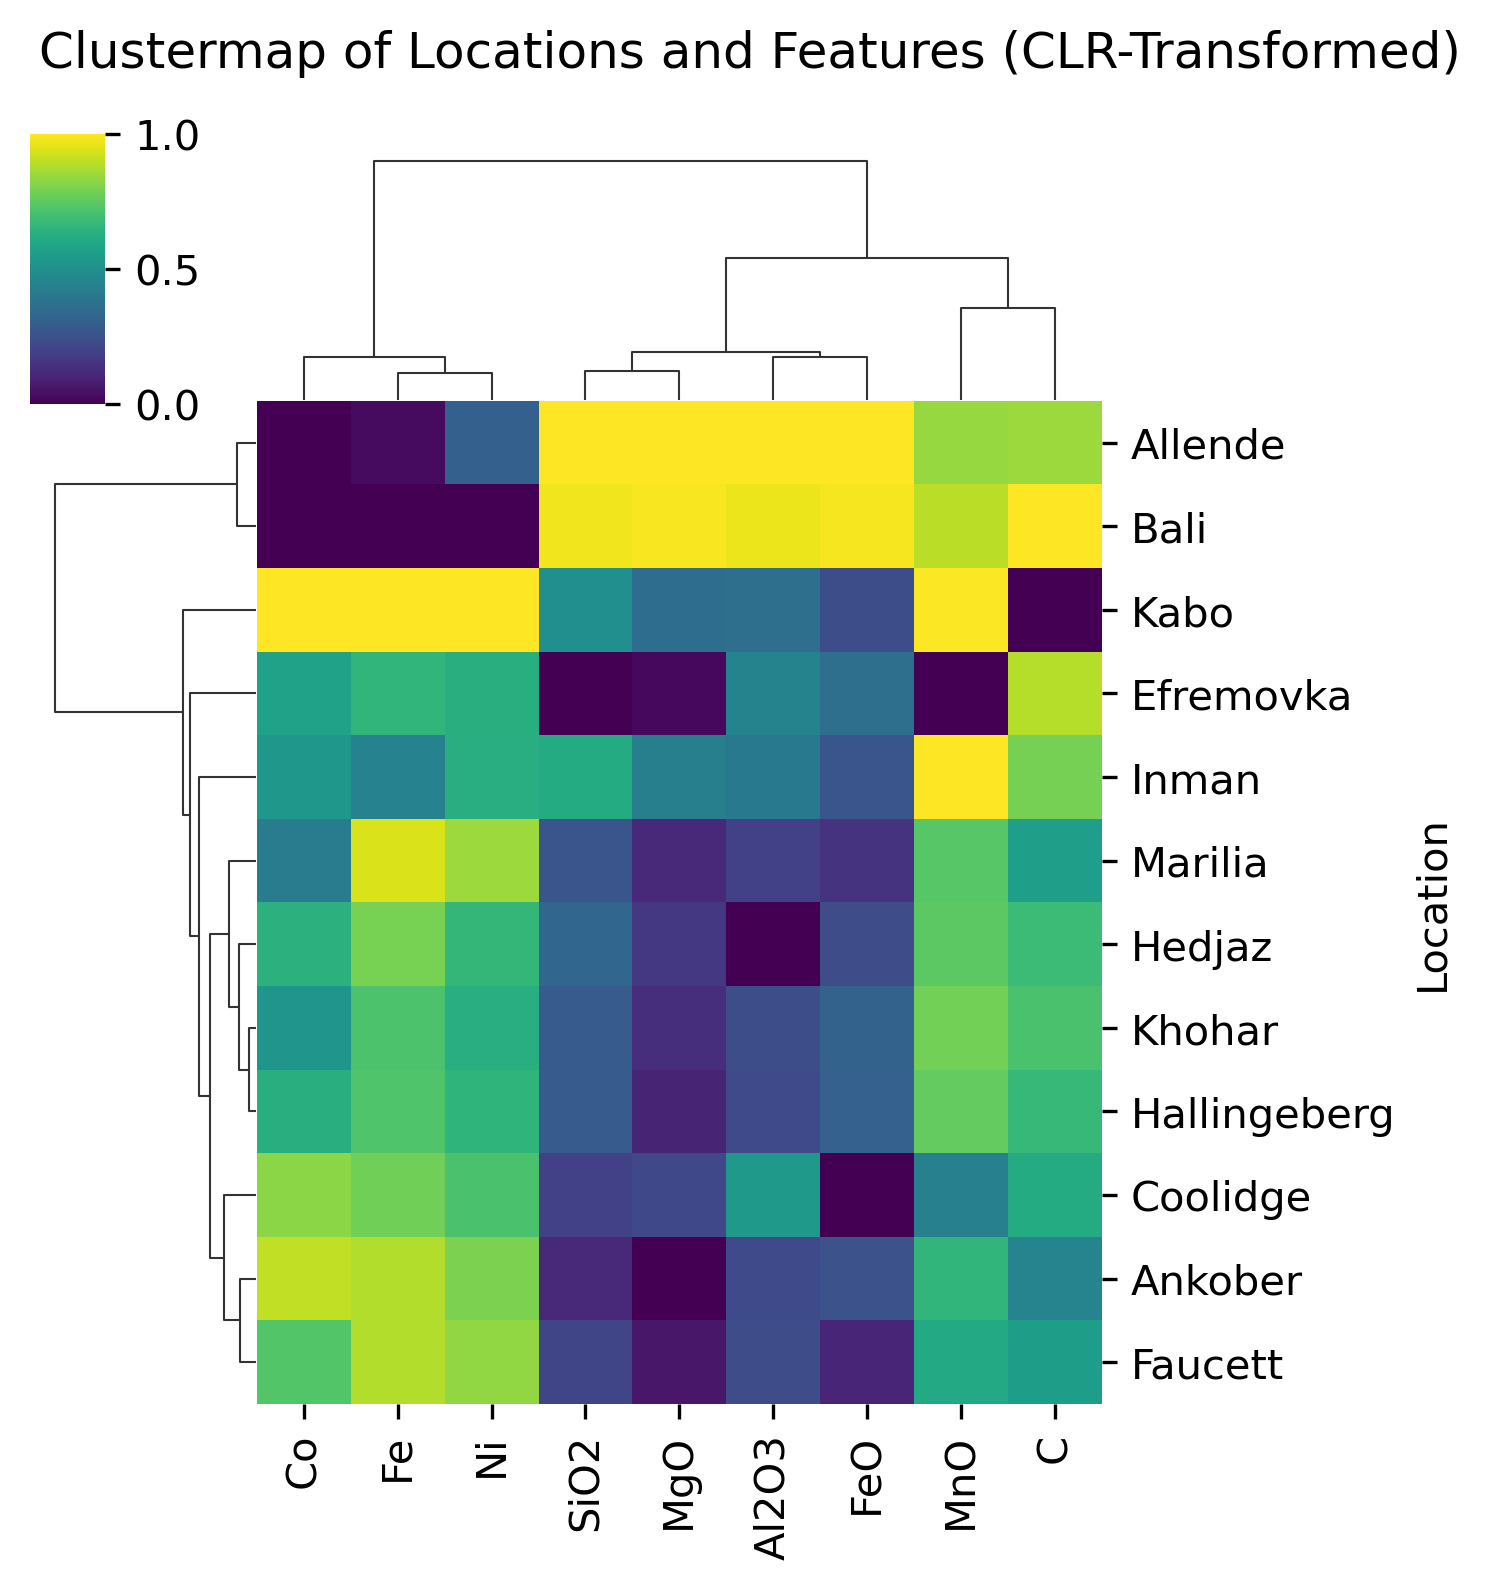
\includegraphics[width=0.4\textwidth]{figures/clustermap.png}
    \caption{Example plot showing the chemical composition of meteorites.}
    \label{fig:clustermap}
\end{figure}


